\FloatBarrier
\chapter{Branching details and small populations}
\label{m:app:branching-details}

The main text uses the binary Galton--Watson process as a compact discrete-time
example.  This appendix retains the calculations that support that example but
would otherwise interrupt the process-and-methods structure: the critical power
laws, the limiting conditional variance, the effect of several founders, and the
discrete rupture calculation.

\section{Critical survival, lifetime and total progeny}
\label{m:app:critical-gw}

At $p=\tfrac12$, the mean population is one at every generation, although
extinction is certain.  The apparent tension is resolved by a heavy tail: a small
fraction of realisations become sufficiently large to hold the unconditional mean
at one.

\begin{proposition}[Critical survival probability]
For the critical binary Galton--Watson process,
\begin{equation}
  S_n\sim\frac{2}{n}
  \qquad(n\to\infty).
  \label{m:eq:critical-Sn}
\end{equation}
\end{proposition}

\begin{proof}
At $p=\tfrac12$, the exact recursion \cref{m:eq:SnIter} becomes
\begin{equation}
  S_{n+1}=S_n-\frac12S_n^2
  =S_n\left(1-\frac{S_n}{2}\right).
  \label{m:eq:critical-recursion}
\end{equation}
Since $S_n\downarrow0$, its reciprocal tends to infinity.  The reciprocal
increments satisfy
\begin{equation}
  \frac{1}{S_{n+1}}-\frac{1}{S_n}
  =\frac{1}{2(1-S_n/2)}\longrightarrow\frac12.
  \label{m:eq:critical-reciprocal-increment}
\end{equation}
Stolz--Ces\`aro applied to $(1/S_n)/n$, equivalently the Ces\`aro limit of the
increments in \cref{m:eq:critical-reciprocal-increment}, gives
$(1/S_n)/n\to1/2$.  This is \cref{m:eq:critical-Sn}.
\end{proof}

Let
\begin{equation}
  T=\inf\{n\geq0:Z_n=0\}
  \label{m:eq:critical-extinction-time}
\end{equation}
be the extinction time.  Since
$T=\sum_{n\geq0}\mathbf 1_{\{T>n\}}$, Tonelli's theorem gives the tail-sum
identity
\begin{equation}
  \ex{T}=\sum_{n=0}^{\infty}\pr{T>n}
  =\sum_{n=0}^{\infty}S_n.
  \label{m:eq:critical-tail-sum}
\end{equation}
The last series has the same divergent tail as $2\sum_n n^{-1}$, and hence
$\ex{T}=\infty$.  Extinction is almost sure, but its expected time is infinite.
Moreover, the decrement in \cref{m:eq:critical-recursion} is exact, so
\begin{equation}
  \pr{T=n+1}=S_n-S_{n+1}=\frac12S_n^2
  \sim\frac{2}{n^2}.
  \label{m:eq:critical-extinction-mass}
\end{equation}

The total progeny
\begin{equation}
  \mathcal T=\sum_{n\geq0}Z_n
  \label{m:eq:total-progeny}
\end{equation}
has a different exponent.  A finite binary genealogy with $k$ division vertices
contains $k+1$ terminal vertices and hence $2k+1$ individuals.  The number of
ordered full binary trees with $k$ division vertices is the Catalan number
\[
  C_k=\frac{1}{k+1}\binom{2k}{k}.
\]
Each such tree has probability $p^k(1-p)^{k+1}$, and therefore
\begin{equation}
  \pr{\mathcal T=2k+1}=C_kp^k(1-p)^{k+1}.
  \label{m:eq:total-progeny-exact}
\end{equation}
At criticality, $C_k\sim4^k/(\sqrt{\pi}k^{3/2})$, so Stirling's formula gives
\begin{equation}
  \pr{\mathcal T=2k+1}
  \sim\frac{1}{2\sqrt{\pi}}k^{-3/2},
  \label{m:eq:total-progeny-asymptotic}
\end{equation}
with zero probability at even values.  The survival, lifetime-mass and
total-progeny exponents are shown together in \cref{m:fig:critical-power-laws}.

\begin{figure}[tbp]
  \centering
  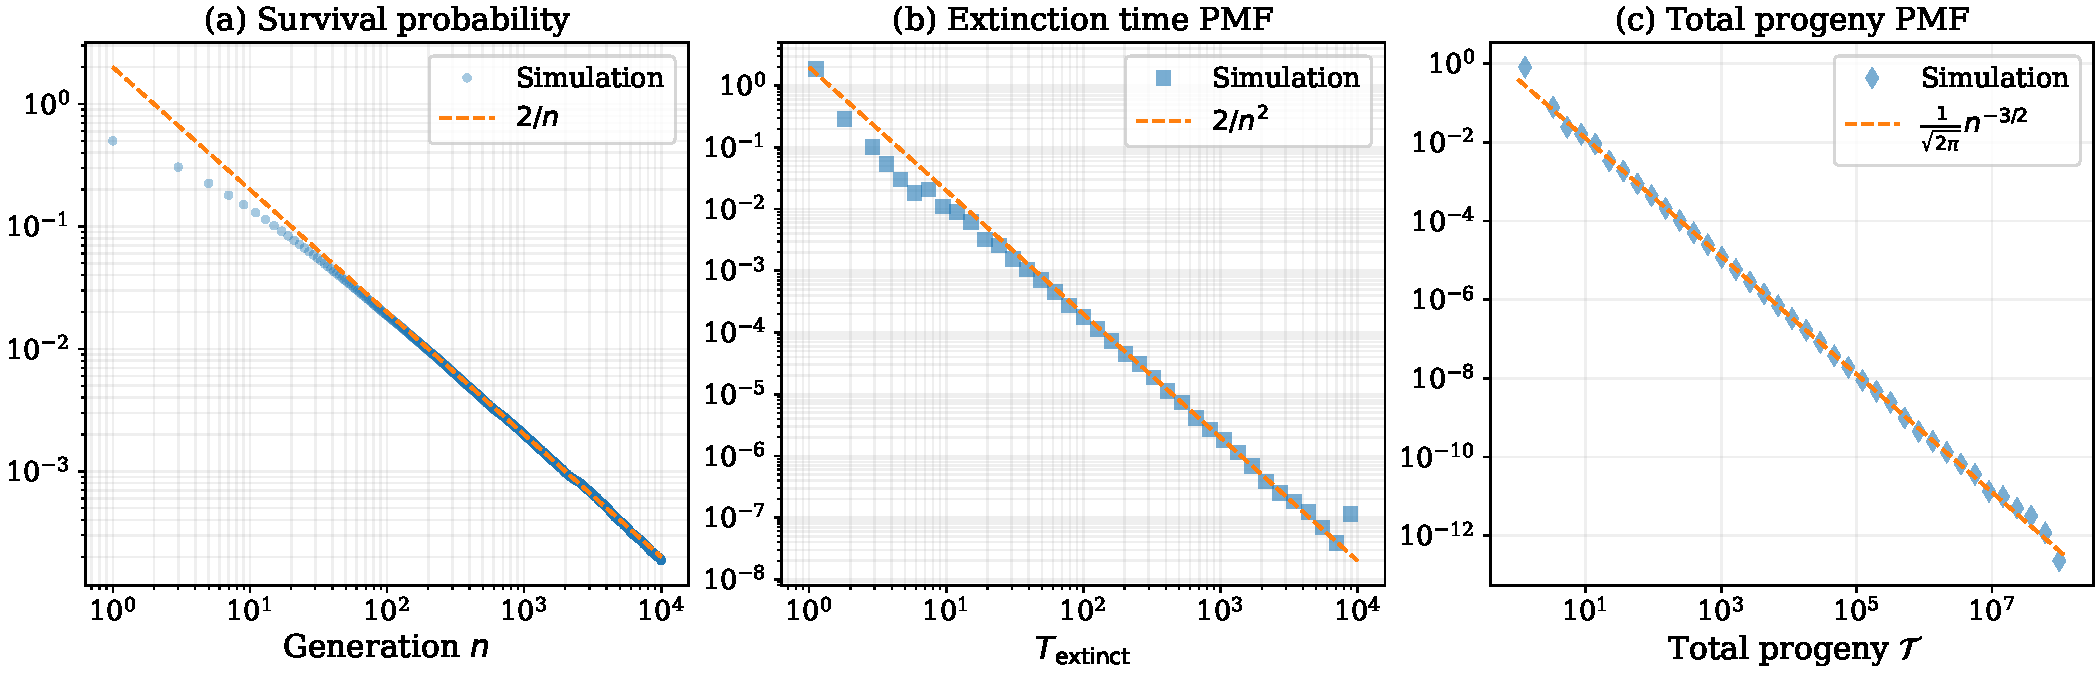
\includegraphics[width=0.97\textwidth]{figures/IMG_ch3/power_law_fixed.pdf}
  \caption{Critical power laws from $10^6$ simulated binary Galton--Watson
  realisations.  From left to right: $S_n\sim2/n$,
  $\pr{T=n}\sim2/n^2$, and the $n^{-3/2}$ total-progeny law on its odd support.
  The first two exponents also follow directly from
  \cref{m:eq:critical-recursion}.}
  \label{m:fig:critical-power-laws}
\end{figure}

\section{The limiting conditional variance}
\label{m:app:conditional-variance}

Let $m=2p$ and write $M_n=\ex{Z_n^2}$.  If $\sigma^2$ is the offspring
variance, then conditional on $Z_n$ the next generation is a sum of $Z_n$
independent offspring counts.  Consequently
\begin{equation}
  \ex{Z_{n+1}^2\mid Z_n}=\sigma^2Z_n+m^2Z_n^2,
\end{equation}
and hence
\begin{equation}
  M_{n+1}=m^2M_n+\sigma^2m^n,
  \qquad M_0=1.
  \label{m:eq:discrete-second-moment-recurrence}
\end{equation}
For the binary offspring law,
$\sigma^2=4p(1-p)=m(2-m)$.  Solving
\cref{m:eq:discrete-second-moment-recurrence} for $m\neq1$ gives
\begin{align}
  \ex{Z_n^2}
  &=m^{2n}+\sigma^2m^{n-1}\frac{1-m^n}{1-m}
  \notag\\
  &=m^n\left(1+\frac{1}{1-m}\right)
    -\frac{m^{2n}}{1-m}.
  \label{m:eq:binary-second-moment}
\end{align}
The second line is specific to the binary variance.  At $n=1$ it returns
$\ex{Z_1^2}=4p$, which checks the sign of the final term.

For $m<1$, divide by $S_n\sim A(p)m^n$ to obtain
\begin{equation}
  \ex{Z_n^2\mid Z_n>0}
  =\frac{\ex{Z_n^2}}{S_n}
  \longrightarrow
  \frac{1}{A(p)}\left(1+\frac{1}{1-2p}\right).
  \label{m:eq:qsd-second-moment}
\end{equation}
Combining this with
$\ex{Z_n\mid Z_n>0}\to1/A(p)$ proves
\cref{m:eq:discrete-conditional-variance}.  These limits are the first two
moments of the binary Yaglom law.  The moment calculation does not itself prove
convergence of the full conditional distribution; that conclusion belongs to the
classical quasi-stationary theory developed for Galton--Watson processes
\cite{Harris1963,Athreya1972}.

\section{Small founding populations}
\label{m:app:small-populations}

For a single founder, the survival and extinction recursions start at $S_0=1$ and
$u_0=0$.  At criticality, survival through two generations is
\begin{equation}
  S_2=\frac12\left(1-\frac14\right)=\frac38.
  \label{m:eq:two-generation-survival}
\end{equation}
The factor $1/2$ requires the founder to divide, while $1-1/4$ requires at least
one of its two descendants to divide in the next generation.  Iteration gives the
early extinction probabilities quoted in \cref{m:sec:founding-bottlenecks}.

\begin{figure}[tbp]
  \centering
  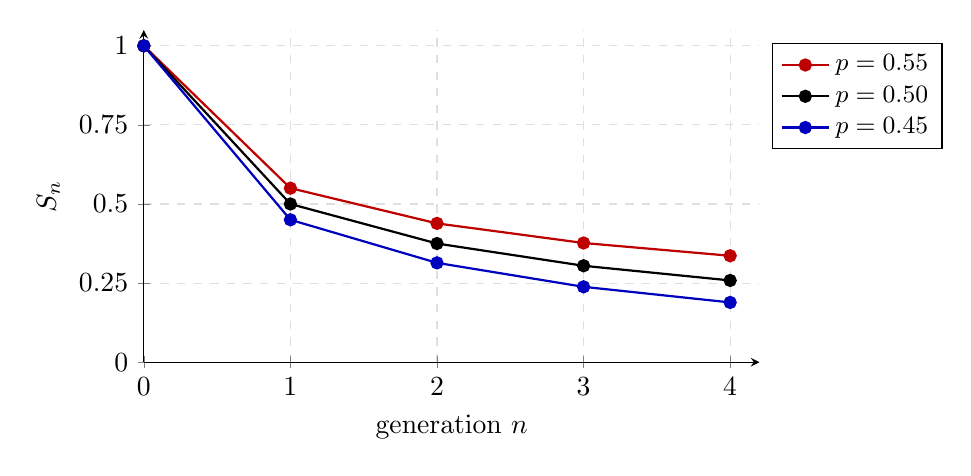
\begin{tikzpicture}
    \begin{axis}[
      width=9.4cm,height=5.8cm,
      axis lines=left,xlabel={generation $n$},ylabel={$S_n$},
      xmin=0,xmax=4.2,ymin=0,ymax=1.05,
      xtick={0,1,2,3,4},ytick={0,0.25,0.5,0.75,1},
      grid=major,grid style={dashed,gray!25},
      legend style={font=\small,at={(1.02,0.96)},anchor=north west}]
      \addplot[red!75!black,thick,mark=*] coordinates
        {(0,1) (1,0.55) (2,0.438625) (3,0.3766719) (4,0.336304)};
      \addlegendentry{$p=0.55$}
      \addplot[black,thick,mark=*] coordinates
        {(0,1) (1,0.5) (2,0.375) (3,0.3046875) (4,0.2582703)};
      \addlegendentry{$p=0.50$}
      \addplot[blue!75!black,thick,mark=*] coordinates
        {(0,1) (1,0.45) (2,0.313875) (3,0.2381546) (4,0.188816)};
      \addlegendentry{$p=0.45$}
    \end{axis}
  \end{tikzpicture}
  \caption{Survival over the first four generations from one founder.  Early
  loss is steep in all three regimes; a modest supercritical advantage does not
  remove the founding bottleneck.}
  \label{m:fig:early-survival}
\end{figure}

For $Z_0=k$, the $k$ descendant trees are independent.  The exact survival law
\cref{m:eq:k-founder-survival} has two useful limits.  When $S_n$ is small and
$kS_n\ll1$,
\begin{equation}
  S_n^{(k)}=1-(1-S_n)^k\sim kS_n,
  \label{m:eq:k-founder-small-survival}
\end{equation}
whereas the full expression must be retained when the cohort makes survival
appreciable.  A larger cohort can postpone extinction at criticality but cannot
prevent it; just above criticality it also raises the probability that at least
one founding lineage belongs to the non-extinguishing set.

\begin{figure}[H]
  \centering
  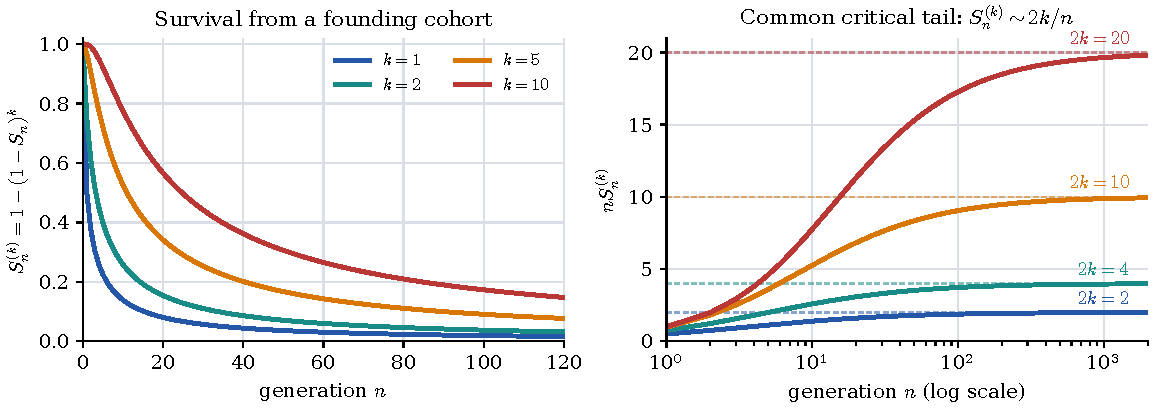
\includegraphics[width=0.94\textwidth]{figures/generated/founder_cohort_survival.pdf}
  \caption{Critical survival from $k$ independent founders.  The left panel
  shows the exact cohort law \cref{m:eq:k-founder-survival}: additional founders
  soften the early bottleneck but do not prevent eventual extinction.  The right
  panel rescales by generation number; the approach to $2k$ displays the common
  tail $S_n^{(k)}\sim2k/n$.}
  \label{m:fig:founder-cohort-survival}
\end{figure}

Conditioning on survival to a late time selects paths after they have been
generated.  Paths with favourable early reproduction are over-represented among
the survivors, so their mean early growth can exceed the unconditional mean even
when the offspring law is time-homogeneous.  This push-of-the-past effect was
identified in longevity and diversity data by Budd and Mann
\cite{Budd2018}.  Here it follows directly from the steep early attrition in
\cref{m:fig:early-survival,m:fig:founder-cohort-survival}: the conditioning
changes the sampled ensemble, not the transition mechanism.

\section{Discrete rupture and the Jensen bound}
\label{m:app:discrete-rupture}

Suppose first that the population doubles deterministically at each generation
until rupture.  Each individual exposed during a step independently initiates
rupture with probability $\kappa\in[0,1]$, and a single initiation ends the
process.  The population exposed during generations $0,\ldots,n-1$ has total size
\[
  1+2+\cdots+2^{n-1}=2^n-1.
\]
The probability of no rupture before generation $n$ is therefore
\begin{equation}
  R_n=(1-\kappa)^{2^n-1},
  \label{m:eq:pure-birth-no-rupture}
\end{equation}
and, conditional on reaching step $n$, the probability of rupture during that
step is
\begin{equation}
  1-(1-\kappa)^{2^{n-1}}.
  \label{m:eq:rupture-at-step}
\end{equation}

When death is allowed, the accumulated exposure is random.  Let
$\widetilde Z_i$ denote the binary Galton--Watson population with rupture switched
off and define
\begin{equation}
  H_n=\sum_{i=0}^{n-1}\widetilde Z_i.
  \label{m:eq:rupture-exposure}
\end{equation}
Conditioning on the whole catastrophe-free genealogy gives the exact identity
\begin{equation}
  \pr{\text{no rupture before }n}
  =\ex{(1-\kappa)^{H_n}}.
  \label{m:eq:no-rupture-expectation}
\end{equation}
The map $h\mapsto(1-\kappa)^h$ is convex, so Jensen's inequality yields
\begin{equation}
  \pr{\text{no rupture before }n}
  \geq(1-\kappa)^{\ex{H_n}}.
  \label{m:eq:no-rupture-jensen}
\end{equation}
With $m=2p$,
\begin{equation}
  \ex{H_n}=\sum_{i=0}^{n-1}m^i
  =
  \begin{cases}
    \dfrac{1-m^n}{1-m},&m\neq1,\\[2mm]
    n,&m=1.
  \end{cases}
  \label{m:eq:mean-rupture-exposure}
\end{equation}
Replacing exposure by its mean is thus a lower bound, not an equality.

Finally, non-rupture is not the same event as survival.  The probability that the
population is both unruptured and non-zero at generation $n$ is
\begin{equation}
  \ex{\mathbf 1_{\{\widetilde Z_n>0\}}(1-\kappa)^{H_n}},
  \label{m:eq:joint-survival-no-rupture}
\end{equation}
for which \cref{m:eq:no-rupture-jensen} does not directly provide a bound.  This
distinction is the discrete counterpart of separating ordinary extinction from
catastrophe in the killed-chain balance \cref{m:eq:bdc-survival-loss}.

\FloatBarrier
